% !TEX program = lualatex
\documentclass[aspectratio=169,professionalfonts]{beamer}
%------------------------- Preamble (beamer) -------------------------%
%   Require LuaLaTeX + --shell-escape (for minted)                    %
%--------------------------------------------------------------------%
\usepackage[spanish]{babel}

% ---------- Fonts (modern look) ----------
\usepackage{fontspec}
\defaultfontfeatures{Ligatures=TeX, Scale=MatchLowercase}
\setmainfont{Inter}       % Sans‑serif body (install ttf–Inter)
\setsansfont{Inter}
\setmonofont{Fira Code}   % Nice mono for code

% ---------- Theme ----------
\usetheme[
  titleformat=smallcaps,
  numbering=fraction,
  progressbar=frametitle   % thin progress line under the title
]{metropolis}              % modern beamer theme
\metroset{block=fill}      % coloured blocks

% ---------- Colours ----------
\definecolor{clblue}{HTML}{005F9E}
\definecolor{clorange}{HTML}{FF9130}
\definecolor{clgrey}{HTML}{F4F4F4}

% ---------- minted ----------
\usepackage{minted}
\setminted{
  fontsize=\footnotesize,
  autogobble,
  breaklines,
  tabsize=2,
  style=monokai,
  linenos
}

% ---------- Custom boxes (tcolorbox) ----------
\usepackage{tcolorbox}
\tcbuselibrary{skins, breakable}
% Warning box
\newtcolorbox{warnbox}{
  colback=clorange!10,
  colframe=clorange!80!black,
  breakable,
  title={\faWarning\quad Advertencia},
  fonttitle=\bfseries,
  left=2mm, right=2mm, top=1mm, bottom=1mm
}
% Information box
\newtcolorbox{infobox}{
  colback=clblue!5,
  colframe=clblue!60!black,
  breakable,
  title={\faInfoCircle\quad Nota},
  fonttitle=\bfseries,
  left=2mm, right=2mm, top=1mm, bottom=1mm
}

% ---------- Icons ----------
\usepackage{fontawesome5}

% ---------- Misc tweaks ----------
\graphicspath{{figures/}}
\setlength{\parskip}{0.5em}
\addto\extrasspanish{\renewcommand{\contentsname}{Índice}}
%--------------------------------------------------------------------%


\usepackage{mwe} % figuras de ejemplo -> example-image

\title[ClústerLab • Día 2]{Redes IP y claves SSH}
\subtitle{Configurar IP estática y generar claves}
\author{Equipo docente ClústerLab}
\date{6 de agosto de 2025}

\begin{document}

%------------------------------ portada ----------------------------
\begin{frame}[plain]
  \titlepage
\end{frame}

%------------------------------ básico de redes -------------------------
\begin{frame}[fragile]{Básico de redes}
  Los computadores y otros dispositivos, para comunicarse entre ellos, necesitan una especie de nombre,
  que sería la \textit{ip address}, o dirección ip (ip: internet protocol).

  La forma más común de ip es la IPv4 (ej: 192.168.0.155).

  La ip se la da la entidad que esté por encima del dispositivo, entonces, un celular recibe su ip de 
  el router o de la antena 4G/5G. El router y la antena reciben su ip de la ISP (internet service provider),
  como Claro o Movistar. Y estas ISP reciben sus ips de organismos mundiales (LACNIC <- ICANN/IANA)
\end{frame}

%------------------------------ network dentro -------------------------
\begin{frame}[fragile]{Dentro una network}
  Generalmente, se le asigna una IP única a cada dispositivo. Y, generalmente, esa IP se mantiene a lo largo del tiempo.
  Para ver la ip que uno tiene, en linux:
  \begin{minted}{bash}
  $ ip a
  \end{minted}
  \begin{center}
    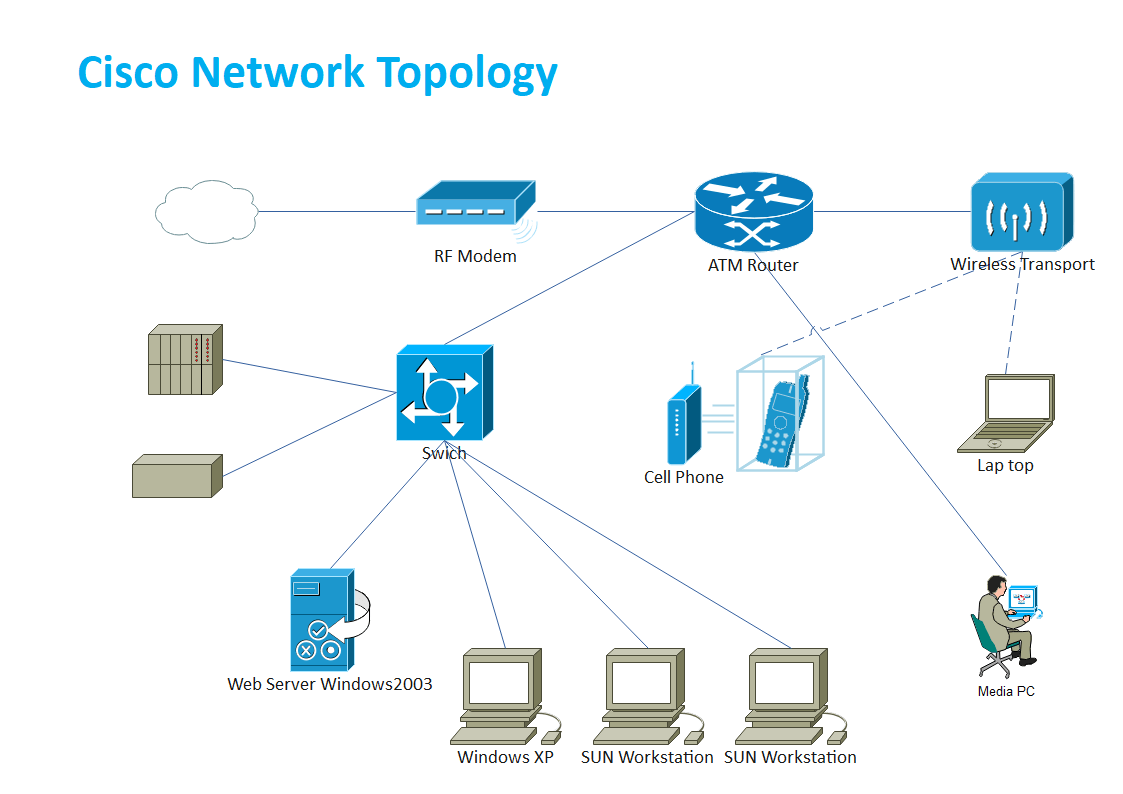
\includegraphics[width=.45\textwidth]{cisco_network_diagram.png}
  \end{center}
\end{frame}

%------------------------------ prueba ip -------------------------
\begin{frame}[fragile]{Verificar conectividad}
  \begin{minted}{bash}
$ ip addr show eth0 | grep 'inet '
$ ping -c3 10.0.0.1
  \end{minted}
  \begin{itemize}
    \item Confirma que la IP asignada se muestre en \texttt{inet}.
    \item Un par de \texttt{ping} verifica la ruta al gateway.
  \end{itemize}
  \begin{center}
    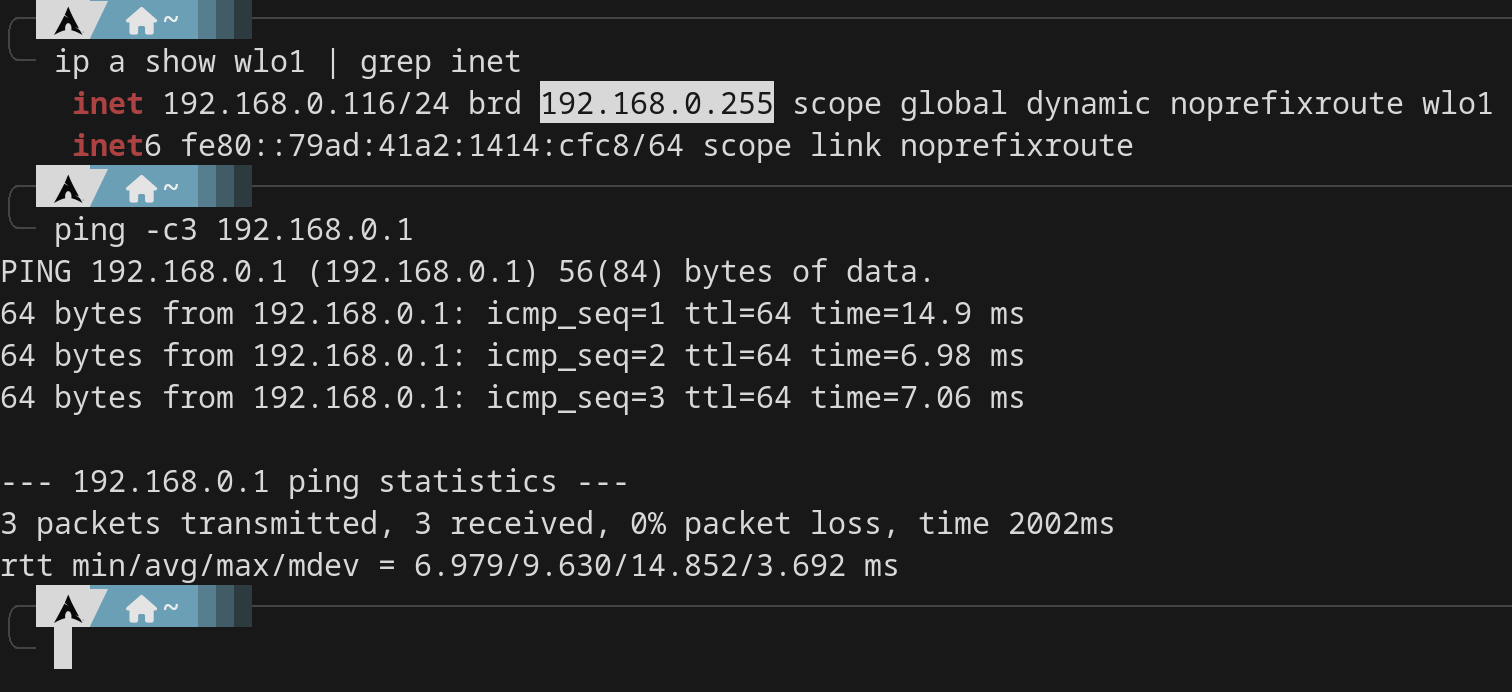
\includegraphics[width=.6\textwidth]{ipping.png}
  \end{center}
\end{frame}

%------------------------------ info ---------------------------
\begin{frame}[fragile]{Info importante}
  \begin{infobox}
    las ip que terminen en \texttt{.0}, \texttt{.1} o \texttt{.255} suelen ser reservadas. Intentar no molestar esas IPs

    \begin{itemize}
      \item red: \texttt{x.x.x.0}
      \item router: \texttt{x.x.x.1}
      \item todos: \texttt{x.x.x.255}
    \end{itemize}
  \end{infobox}
  \begin{infobox}
    Intentar usar el comando \texttt{ping} siempre con \texttt{-c4} u otro número bajo. Sino, se quedará ejecutando hasta que sea interrumpido.

    \texttt{ping -c4}
  \end{infobox}
\end{frame}

%------------------------------ ssh test ---------------------------
\begin{frame}[fragile]{Probar acceso SSH}
  \begin{minted}{bash}
$ ssh pi@10.0.0.21 hostname
$ ssh pi@10.0.0.21 hostnamectl
  \end{minted}
  Si la autenticación funciona, verás el nombre de tu Pi en la salida.
  \begin{minted}{bash}
# Opcional en ~/.ssh/config
Host rpi21
  HostName 10.0.0.21
  User pi
  \end{minted}
  Entonces basta con ejecutar:
  \begin{minted}{bash}
$ ssh rpi21
  \end{minted}
\end{frame}

%------------------------------ sin contraseña --------------------------
\begin{frame}[fragile]{Usar ssh sin contraseña}
  Útil para conexiones frecuentes o contraseñas complejas. Sólo necesitas usar la contraseña una única vez.
  \begin{enumerate}
    \item Primero, generar claves, una pública y una privada.
    \begin{minted}{bash}
     $ ssh-keygen -t ed25519
    \end{minted}
    \item Generará 2 archivos,
    \begin{itemize}
      \item \texttt{\textasciitilde/.ssh/id\_ed25519} clave \textbf{privada}. Nunca compartir.
      \item \texttt{\textasciitilde/.ssh/id\_ed25519.pub} clave \textbf{pública}. Esta se copiará al servidor.
    \end{itemize}
    \item Usar el commando \texttt{ssh-copy-id} para copiar la clave pública al servidor.
    \begin{minted}{bash}
     $ ssh-copy-id pi@10.0.0.21
    \end{minted}
    \item Se te pedirá la contraseña una única vez, y la clave pública será añadida a \texttt{\textasciitilde/.ssh/authorized\_keys} del servidor.
  \end{enumerate}
\end{frame}

%------------------------------ claves SSH -------------------------
\begin{frame}[fragile]{Usar ssh sin contraseña}
  \begin{minted}{bash}
# Genera un par RSA de 4096 bits con comentario
$ ssh-keygen -t rsa -b 4096 -C "tu@correo"
# Copia la clave pública a la Raspberry Pi
$ ssh-copy-id pi@10.0.0.21
  \end{minted}
  \begin{infobox}
  La autenticación sin contraseña simplifica el uso de \texttt{scp} y \texttt{rsync}. Protege tu clave privada (\texttt{\textasciitilde/.ssh/id\_rsa}) con permisos 600.
  \end{infobox}
\end{frame}

%------------------------------ puertos %---------------------------
\begin{frame}[fragile]{Puertos Comúnes}
  \begin{itemize}
    \item \texttt{21} es el puerto ftp (file transfer)
    \item \texttt{22} es el puerto ssh (conexión remota)
    \item \texttt{80} es el puerto http (página web)
    \item \texttt{443} es el puerto https (página web segura)
  \end{itemize}
\end{frame}

%------------------------------ nmap scan --------------------------
\begin{frame}[fragile]{Descubrir vecinos con \texttt{nmap}}
  Instala la herramienta y explora quién está conectado:
  \begin{minted}{bash}
$ sudo apt install -y nmap
$ nmap -sn 10.0.0.0/24          # escaneo rápido de hosts
$ nmap -p 22 --open 10.0.0.0/24 # encontrar servicios SSH activos
  \end{minted}
  \begin{itemize}
    \item La opción \texttt{-sn} (ping scan) lista IP y latencias.
    \item Usa \texttt{-p} para verificar puertos específicos como SSH.
  \end{itemize}
\end{frame}


%------------------------------ nmap opciones ----------------------
\begin{frame}[fragile]{Opciones útiles de \texttt{nmap}}
  \begin{minted}{bash}
$ nmap -A 10.0.0.0/24       # detección de servicios y SO
$ nmap --open -p 80 10.0.0.* # buscar servidores web
  \end{minted}
  \begin{itemize}
    \item \texttt{-A} entrega información detallada y requiere más tiempo.
    \item Limita el rango si la red está muy concurrida.
  \end{itemize}
\end{frame}

\end{document}